%%%%%%%%%%%%%%%%%%
% Based on https://github.com/jdavis/latex-homework-template
%%%%%%%%%%%%%%%%%%

\documentclass{article}

\usepackage{fancyhdr}
\usepackage{extramarks}

\usepackage{amsmath}
\usepackage{amsthm}
\usepackage{amsfonts}

\usepackage{tikz}
\usepackage[plain]{algorithm}
\usepackage{algpseudocode}

\usetikzlibrary{automata,positioning}

\usepackage{wrapfig}

\usepackage{lipsum}

%for urls
\usepackage{hyperref}
\hypersetup{
	colorlinks = true,
	linkcolor = teal,
	anchorcolor = teal,
	citecolor = teal,
	filecolor = teal,
	urlcolor = teal
}

%%%%%% Basic Document Settings %%%%%%%%%

\topmargin=-0.45in
\evensidemargin=0in
\oddsidemargin=0in
\textwidth=6.5in
\textheight=9.0in
\headsep=0.25in

\linespread{1.1}

%%%%%%%%%%%%%%%%%% Homework Details %%%%%%%%%%%%%%%
% University Seal
% Title
% Due date
% University
% Class
% Instructor
% Author
% Author ID 
\newcommand{\hmwkSeal}{images/logo.png}
\newcommand{\hmwkTitle}{Assignment\ \#2}
\newcommand{\hmwkDueDate}{April 30, 2023}
\newcommand{\hmwkClass}{Neural Networks \& Representation Learning (CS-587)}
\newcommand{\hmwkClassInstructor}{Ass. Prof. N. Komontakis}
\newcommand{\hmwkUniversity}{University of Crete \\Department of Computer Science}
\newcommand{\hmwkAuthorName}{Nikolaos Kougioulis}
\newcommand{\hmwkAuthorID}{ID 1285}


%fancyhdr
\pagestyle{fancy}
\lhead{\hmwkAuthorName\ (\hmwkAuthorID)} %left head
%\chead{\hmwkClass\ \hmwkTitle} %center head
%\rhead{\date{\today}} %right head
\rhead{\hmwkTitle} 
\lfoot{\lastxmark}
\cfoot{\thepage}

\renewcommand\headrulewidth{0.4pt}

% Create Problem Sections %

\newcommand{\enterProblemHeader}[1]{
	\nobreak\extramarks{}{Problem \arabic{#1} continued on next page\ldots}\nobreak{}
	\nobreak\extramarks{Problem \arabic{#1} (continued)}{Problem \arabic{#1} continued on next page\ldots}\nobreak{}
}

\newcommand{\exitProblemHeader}[1]{
	\nobreak\extramarks{Problem \arabic{#1} (continued)}{Problem \arabic{#1} continued on next page\ldots}\nobreak{}
	\stepcounter{#1}
	\nobreak\extramarks{Problem \arabic{#1}}{}\nobreak{}
}

\setcounter{secnumdepth}{0}
\newcounter{partCounter}
\newcounter{exerciseCounter}
\setcounter{exerciseCounter}{1}
\nobreak\extramarks{Problem \arabic{exerciseCounter}}{}\nobreak{}

% Homework Problem Environment %
% This environment takes an optional argument. When given, it will adjust the problem counter. This is useful for when the problems given for your
% assignment aren't sequential. See the last 3 problems of this template for an example.
%

\newcommand{\enterExerciseHeader}[1]{
	\nobreak\extramarks{}{Exercise \arabic{#1} continued on next page\ldots}\nobreak{}
	\nobreak\extramarks{Exercise \arabic{#1} (continued)}{Exercise \arabic{#1} continued on next page\ldots}\nobreak{}
}

\newcommand{\exitExerciseHeader}[1]{
	\nobreak\extramarks{Exercise \arabic{#1} (continued)}{Exercise \arabic{#1} continued on next page\ldots}\nobreak{}
	\stepcounter{#1}
	\nobreak\extramarks{Exercise \arabic{#1}}{}\nobreak{}
}

\newenvironment{Exercise}[1][-1]{
	\ifnum#1>0
	\setcounter{exerciseCounter}{#1}
	\fi
	\section{Exercise \arabic{exerciseCounter}}
	\setcounter{partCounter}{1}
	\enterExerciseHeader{exerciseCounter}
}{
	\exitExerciseHeader{exerciseCounter}
}

% Title Page %
\title{
	\centering
	\includegraphics[height=1.5in]{\hmwkSeal}
	
	\vspace{1in}
	\textmd{\textbf{\hmwkClass\ \hmwkTitle}}\\
	
	\normalsize\vspace{0.1in}\small{Due\ on\ \hmwkDueDate}\\
	
	\vspace{0.1in}
	\large{\textit{\hmwkClassInstructor}} \\
	\vspace{0.5in}
	
	\large{\hmwkUniversity}
	
	\vspace{3in}
	
	\author{\textbf{\hmwkAuthorName} (\hmwkAuthorID)}
	\date{\today}
}

% Various Helpers %
\newcommand{\alg}[1]{\textsc{\bfseries \footnotesize #1}}
% For derivatives
\newcommand{\deriv}[1]{\frac{\mathrm{d}}{\mathrm{d}x} (#1)}
% For partial derivatives
\newcommand{\pderiv}[2]{\frac{\partial}{\partial #1} (#2)}
% Integral dx
\newcommand{\dx}{\mathrm{d}x}
\newcommand{\E}{\mathbb{E}}
\newcommand{\Var}{\mathrm{Var}}
\newcommand{\Cov}{\mathrm{Cov}}
\newcommand{\Bias}{\mathrm{Bias}}
\newcommand{\Prob}{\mathbb{P}}

\def\code#1{\texttt{#1}}

%for code listings
\usepackage{listings}
\usepackage{xcolor}

\definecolor{codegreen}{rgb}{0,0.6,0}
\definecolor{codegray}{rgb}{0.5,0.5,0.5}
\definecolor{codepurple}{rgb}{0.58,0,0.82}
\definecolor{backcolour}{rgb}{0.99,0.99,0.99}

\lstdefinestyle{mystyle}{
	backgroundcolor=\color{backcolour},   
	commentstyle=\color{codegreen},
	keywordstyle=\color{magenta},
	numberstyle=\tiny\color{codegray},
	stringstyle=\color{codepurple},
	basicstyle=\ttfamily\footnotesize,
	breakatwhitespace=false,         
	breaklines=true,                 
	captionpos=b,                    
	keepspaces=true,                 
	numbers=left,                    
	numbersep=5pt,                  
	showspaces=false,                
	showstringspaces=false,
	showtabs=false,                  
	tabsize=2
}

\lstset{style=mystyle}

%for right and left arrow (used in forward and backward pass plots)
\usetikzlibrary{arrows.meta}

%for arranging figures
\usepackage{subcaption}
\begin{document}
	
	\maketitle
	
	\pagebreak
	
	\subsection{Assignment 2a}
	
	The task of part A of Assignment 2 is to get started with the TensorFlow library and its components (more precisely, version 1.15 of TensorFlow on Python 3.6) and compute the gradient using forward and backward propagation. \\
	
	\begin{itemize}
		\item \textbf{Question:} What is the functionality of upstream? Answer it in your report. \\
	
	The keyword \textit{upstream} in the TensorFlow library (up+stream) refers to the flow of data and operations in the computational graph of the neural network, in the way that the output of a layer is the input of the next layer etc. This concept allows us to describe the flow of data in a neural network model without specifically referring to a particular TensorFlow module \footnote{\url{https://www.tensorflow.org/api_docs/python/tf/custom_gradient}}.
	
	\item \textbf{Question:} For the one-variable function $y(x) = \frac{\sin x }{x}$: i) design the computational graph ii) compute the derivative for the backpropagation process by hand  \\
	
	i) The computational graph for the function $\frac{\sin x}{x}$ is shown in Figure 1. \\
	
	ii) During the forward pass, we have 
	
	$$F(x) \equiv \sin x \cdot \frac{1}{x} \equiv \sin w_1 \cdot \frac{1}{w_1} \equiv w_2 \cdot w_3 \equiv w_4 $$
	
	\tikzstyle{var}=[shape=rectangle,draw=orange!55,fill=yellow!20]
	\tikzstyle{comp}=[shape=circle,draw=red!55, fill=red!20]
	\tikzstyle{lightedge}=[<-,dotted]
	\tikzstyle{mainedge}=[<-,thick]
	
	\begin{figure}
		\centering
		\tikzstyle{mainedge}=[<-,thick,>=stealth]
		\label{fig:1}
		\begin{tikzpicture}[]
			\node[var] (n1) at (0,-3) {$x$}; 
			\node[comp] (n2) at (-1,-1) {$\sin$}
			%edge [mainedge] node[left] {$\phantom{()}$} (n1); % empty node for alignment
			edge [mainedge] node[left] {$w_1^a$} (n1);
			\node[comp] (n3) at (1,-1) {$\frac{1}{x}$}
			edge [mainedge] node[right] {$w_1^b$} (n1);
			\node[comp] (n4) at (0, 1) {$\cdot$}
			edge [mainedge] node[left] {$w_2$} (n2)
			edge [mainedge] node[right] {$w_3$} (n3);
			\node[var] (n5) at (0,2) {$F(x) = \frac{\sin x}{x}$};
			\draw[->,thick] (n4) -- node[above] {$\phantom{()}$} (n5);
			
		    \draw[-Triangle, very thick](-3, -3) -- (-3, 0)
			node[midway,left] {Forward pass};
			\draw[-Triangle, very thick] (3,0) -- (3,-3) 
			node[midway,right] {Backward pass};
		\end{tikzpicture}
	\caption{Computational graph of the function $\displaystyle F(x) = \frac{\sin x}{x}$. After decomposing the function during the forward pass, backpropagation computes the derivative values using the chain rule on the successors of each node in the DAG.}
	\end{figure}
  
   During the backward pass, we obtain using the chain rule 
   
   $$\overline{F} = \overline{w_4} = 1 ~\text{(seed)}$$
   
   $$\overline{w}_3 = \frac{\partial F}{\partial w_3} = \frac{\partial F}{\partial w_4}    \frac{\partial w_4}{\partial w_3} = \overline{w}_4 \cdot w_2$$
   
   $$\overline{w}_2 = \frac{\partial F}{\partial w_2} = \frac{\partial F}{\partial w_4}    \frac{\partial w_4}{\partial w_2} = \overline{w}_4 \cdot w_3$$
   
   $$\overline{w_1}^a = \overline{w_2} \cdot \cos w_1$$
   
   $$\overline{w_1}^b = \overline{w_3} \cdot \left( -\frac{1}{w^2_1} \right)$$
   
   $$\overline{x} = \frac{\partial F}{\partial x} = \overline{w_2} \cos x + \overline{w_3} \cdot \left( - \frac{1}{x^2} \right) = \overline{w_4} w_3 \cos x - \overline{w_4} w_2 \frac{1}{x^2} = 1 \cdot \frac{1}{x} \cos x - \sin x \cdot \frac{1}{x^2} $$
   
   That is,
   
   $$\nabla_x F = \frac{\partial F}{\partial x} = \frac{1}{x} \cos x - \sin x \frac{1}{x^2} $$
   
   which is the same as computing the derivative analytically.
   
	\pagebreak
	
	\item \textbf{Question: } For the two-variable function $f(x,y) = a x^2 +b xy + c y^2$: i) design the computational graph by hand - also include the partial derivatives $\frac{\partial f}{\partial x}$, $\frac{\partial f}{\partial y}$. \\
	
	The computational graph is shown in Figure 2. For the partial derivatives $\frac{\partial F}{\partial x}$, $\frac{\partial F}{\partial y}$, using the chain rule, we need to compute (no computation is asked by the exercise - just including the formulas)
	
	$$\frac{\partial F}{\partial x} = \frac{\partial F}{\partial w_{13}} \frac{\partial w_{13}}{\partial w_{11}} \frac{\partial w_{11}}{\partial w_7} \frac{\partial w_7}{\partial w_1} \frac{\partial w_1}{\partial x} + \frac{\partial F}{\partial w_{13}} \frac{\partial w_{13}}{\partial w_{10}} \frac{\partial w_{10}}{\partial w_3} \frac{\partial w_3}{\partial x}$$
	
	$$\frac{\partial F}{\partial y} = \frac{\partial F}{\partial w_{13}} \frac{\partial w_{13}}{\partial w_{10}} \frac{\partial w_{10}}{\partial w_5} \frac{\partial w_5}{\partial w_y} + \frac{\partial F}{\partial w_{12}} \frac{\partial w_{12}}{\partial w_{8}} \frac{\partial w_{8}}{\partial w_2} \frac{\partial w_2}{\partial y}$$
	
	    \begin{figure}
		\centering
		\label{fig:2}
		\tikzstyle{mainedge}=[<-,thick,>=stealth]
		
		\begin{tikzpicture}[]
			\node[var] (n0) at (-3,1) {$\alpha$};
			\node[var] (n1) at (-3,-1) {$x$};
			\node[var] (n2) at (-3,-3) {$b$};
			\node[var] (n3) at (-3,-6) {$y$};
			\node[var] (n4) at (-3,-9) {$c$};
			\node[comp] (n5) at (-1, -1) {$x^2$}
			edge [mainedge] node[above] {$w_1$} (n1);
			\node[comp] (n6) at (-1, -6) {$y^2$}
			edge [mainedge] node[above] {$w_2$} (n3);
			\node[comp] (n7) at (-1,-3) {$\times$}
			edge [mainedge] node[left] {$w_3$} (n1)
			edge [mainedge] node[above] {$w_4$} (n2)
			edge [mainedge] node[left] {$w_5$} (n3);
			\node[comp] (n8) at (1, 0) {$\times$}
			edge [mainedge] node[above] {$w_6$} (n0)
			edge [mainedge] node[right] {$w_7$} (n5);
			\node[comp] (n9) at (1, -7) {$\times$}
			edge [mainedge] node[above] {$w_8$} (n6)
			edge [mainedge] node[above] {$w_9$} (n4);
			\node[comp] (n10) at (3, -3) {$+$}
			edge [mainedge] node[above] {$w_{10}$} (n7)
			edge [mainedge] node[left] {$w_{11}$} (n8)
			edge [mainedge] node[left] {$w_{12}$} (n9);
			\node[var] (fin) at (7,-3) {$F(x,y) = \alpha x^2 + \beta xy + c y^2$};
			\draw[->,thick] (n10) -- node[above] {$w_{13}$} (fin);
			
			\draw[-Triangle, very thick](3, 0) -- (6, 0)
			node[midway,above] {Forward pass};
			\draw[-Triangle, very thick] (3,-6) -- (6,-6) 
			node[midway,above] {Backward pass};
		\end{tikzpicture}
		\caption{Computational graph of the function $f(x,y) = ax^2 + bxy + cy^2$.}
		
	\end{figure}

    \newpage 
    
    \item \textbf{Question: } For the function $F(x) = \log(1+e^{x})$, design the computational graph (include it in your report). \\
    	
	\begin{figure}
		\centering
		\label{fig:3}
		\tikzstyle{mainedge}=[<-,thick,>=stealth]
		\begin{tikzpicture}[]
			\node[var] (n1) at (-3,0) {$x$};
			\node[var] (n2) at (-3,-2) {$1$};
			\node[comp] (n3) at (0,0) {$\exp$}
			edge [mainedge] node[left] {$$} (n1);
			\node[comp] (n4) at (2,-1) {$+$}
			edge [mainedge] node[left] {$$} (n2)
			edge [mainedge] node[left] {$$} (n3);
			\node[comp] (n5) at (4,-1) {$\log$}
			edge [mainedge] node[left] {$$} (n4);
			\node[var] (n6) at (7,-1) {$F(x) = \log \left( 1 + e^x \right)$};
			\draw[->,thick] (n5) -- node[above] {$\phantom{()}$} (n6);
			
		    \draw[-Triangle, very thick](3, 0) -- (6, 0)
			node[midway,above] {Forward pass};
			\draw[-Triangle, very thick] (6,-2) -- (3,-2) 
			node[midway,above] {Backward pass};
		\end{tikzpicture}
	\caption{Computational graph of the function $F(x) = \log(1+e^x)$}
	
	\end{figure}

    The computational graph is shown in Figure 3. 
        
    \end{itemize}

    \pagebreak
    
    \subsection{Assignment 2b}
    	
    The task in this part of the assignment is to perform supervised learning using neural networks (on image recognition) using the \code{load\_digits} dataset, in TensorFlow and Tensorboard. \\
    
    The dataset contains 1,797 samples of 8x8 images of handwritten digits, where and each pixel in the image is represented by a grayscale value ranging from 0 to 16. With a total of output variables (target)  being 10 (numbers 0,1,\ldots,9). \\
    
    We begin as asked by creating a one hidden layer model, with default parameters \code{batch\_size = 32}, \code{hid\_size = 1}, \code{learning\_rate = 0.01}, \code{num\_epochs = 10} and the Relu activation function, with no regularization term. The resulting computational graph, generated using Tensorboard, is shown in Figure 4. By default, the TensorBoard library shows the op-level graph, with data flowing from bottom to top, so it is upside down compared to the code. It also allows us to view not only the main graph but the auxiliary nodes as well (right part of the figure). \\
    
    The cross entropy loss over the number of iterations is shown in Figure 5, tracked during training using Tensorboard. Notice how initially there is a sudden drop in the loss and after a number of iterations it begins oscillating around a fixed point, where no increment of iterations and number of epochs can further lower the loss of the model. \\
    
    \begin{figure}
    		\centering
    		\includegraphics[width=\textwidth]{images/png.png}
    		\caption{Computational Graph of NN.}
    	\end{figure}
    	
    	\begin{figure}
    		\centering
    		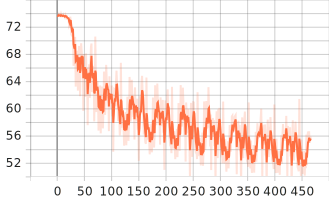
\includegraphics[width=0.4\textwidth]{images/cross_entropy_loss.pdf}
    		\caption{Plot of the cross-entropy loss of the model in Part 2. Bold colored plot is shown with a smoothing value of 0.6.}
    	\end{figure}

    \begin{figure}
    	\begin{subfigure}{0.55\textwidth}
    		\centering
    		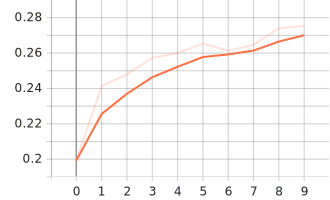
\includegraphics[width=\textwidth]{images/train_accuracy.pdf}
    		\caption{Train accuracy, exported from Tensorboard of the model in Part 2. Bold colored plot is shown with a smoothing value of 0.6.}
    	\end{subfigure}
    	\captionsetup{justification=centering}
    	\hspace{0.05\textwidth}
    	\begin{subfigure}{0.45\textwidth}
    		\centering
    		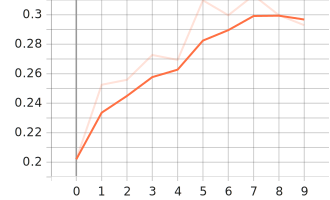
\includegraphics[width=\textwidth]{images/test_accuracy.pdf}
    		\caption{Test accuracy, exported from Tensorboard of the model in Part 2. Bold colored plot is shown with a smoothing value of 0.6.}
    	\end{subfigure}
    	\caption{Figures}
    \end{figure}

For Part 3 of the assignment, we attempt to fine-tune the hyperparameters of our model in order to maximize the test accuracy, while also adding a regularization term. Due to the high number of combinations between each hyperparameter (batch size, hidden layer size, learning rate, number of epochs and regularization strength) we have opted to fix the activation function instead of inserting it as a hyperparameter as well. \\

We perform hyperparameter tuning using random walk search, that is, out of 160 randomly selected parameter configurations select the one that maximizes our test accuracy. Of the RELu, $\tanh$ and sigmoid activation functions, the first two performed slightly worse, hence we opted to only use the sigmoid activation function. \\

After selecting and evaluating the random configurations, our optimal yields a test set accuracy of 0.9259 using the following parameters: \\

\begin{itemize}
	\item activation function: sigmoid
	\item batch size: 64
	\item hidden size: 30
	\item best learning rate: 0.05
	\item best regularization strength: 0.001
	\item best num epochs: 20
\end{itemize}

While training, we keep monitoring the cross-entropy loss of the fine-tuned model in Tensorboard. Notice the spike at the first iterations and then a decrement close to zero during the training process. This is because at the beginning of training, the parameters of the model are randomly initialized and it is more likely to make random predictions.

	\begin{figure}
	\centering
	\includegraphics[width=0.45\textwidth]{images/tuned_loss.png}
	\caption{Plot of the cross-entropy loss of the fine-tuned model, exported from Tensorboard. Bold colored plot is shown with a smoothing value of 0.6.}
\end{figure}


\begin{thebibliography}{}
	\bibitem{goodfellow2016} Goodfellow, I., Bengio, Y., \& Courville, A. (2016). \textit{Deep learning}. MIT Press.
\end{thebibliography}

\end{document}
